\documentclass[11pt]{article}
\usepackage[margin=1in]{geometry}
\usepackage{amsmath,amssymb,booktabs,graphicx,hyperref}
\title{Which Step Should You Check? An Empirical Study of Decision-Risk-Aware Verification Selection for Reasoning Chains}
\author{Burhava project}
\date{Draft}
\begin{document}
\maketitle

\begin{abstract}
% Fill ONLY with numbers from results/summaries/*.json (see docs/RESULTS.md).
We study which premise or inference step of a reasoning chain to verify under a budget.
The selection rule is classical Value of Information (VoI): verify the atom whose
verdict is expected to reduce the loss of the final accept/reject/abstain decision
the most per unit cost. We make no claim that this rule is new; we test empirically,
under a pre-registered protocol, whether it beats confidence-based selection and
whether the advantage survives estimation noise. % generated by scripts/make_paper_numbers.py
In oracle synthetic experiments, lookahead VoI lowers mean decision loss relative to lowest-confidence-first in all four graph structures (e.g. mixed graphs, budget 2: +0.112 [+0.107, +0.116]). The advantage survives calibration error (ECE 0.10, verifier error 5\%: +0.065 [+0.052, +0.077]), but a loss-blind influence score matches it at budgets of 1--2 and beats it at 3--5, and the advantage disappears once 5\% of dependency edges are wrong. A second pre-registered study confirms that decision-aware selection adds nothing over influence-based selection (+0.0000 [-0.0003, +0.0003]), and that averaging over plausible graphs restores a gain at 10\% edge error (+0.016 [+0.002, +0.030]) but not at 25\%.

\end{abstract}

\section{Introduction}
% Problem: verification budgets; confidence-based selection; decision loss is what matters.
% Contribution: empirical, pre-registered comparison; boundary conditions under noise.

\section{Related work}
% Value of information: Howard 1966; Krause \& Guestrin 2009.
% Adaptive submodularity: Golovin \& Krause 2011; non-submodular VoI surrogates: Chen et al. 2015 (DiRECt).
% Stochastic Boolean function evaluation: Deshpande, Hellerstein \& Kletenik 2014.
% Troubleshooting: Heckerman, Breese \& Rommelse 1995. DTProbLog: Van den Broeck et al. 2010.
% LLM verification / claim-level confidence: four arXiv items from the brief -- VERIFY before citing.
% Benchmarks: RuleTaker (Clark et al. 2020), ProofWriter (Tafjord et al. 2021), PrOntoQA (Saparov \& He 2023).

\section{Method: verification selection as a VoI instance}
% Notation from docs/MATH.md: atoms $Z_i$, AND/OR rules, verifier errors $\alpha_i,\beta_i$,
% loss $L(d,y)$, Bayes risk $\rho$, set risk $R(S)$, marginal value $\Delta_i(S)$.
% Arms 9 (one-step $\Delta_i/c_i$) and 10 (two-step lookahead when stalled); AND counterexample.

\section{Experiments}
\subsection{Stage A: oracle synthetic}
% Grid, two generators, paired design, pre-registration (docs/PREREGISTRATION.md).
\begin{tabular}{lcc}\toprule
Structure & Gain of arm 10 over arm 3 (95\% CI) & $n$ \\\midrule
chain & +0.030 [+0.028, +0.032] & 64000 \\
and & +0.003 [+0.002, +0.003] & 64000 \\
or & +0.082 [+0.078, +0.087] & 64000 \\
mixed & +0.112 [+0.107, +0.116] & 64000 \\
\bottomrule\end{tabular}

\begin{figure}[t]\centering
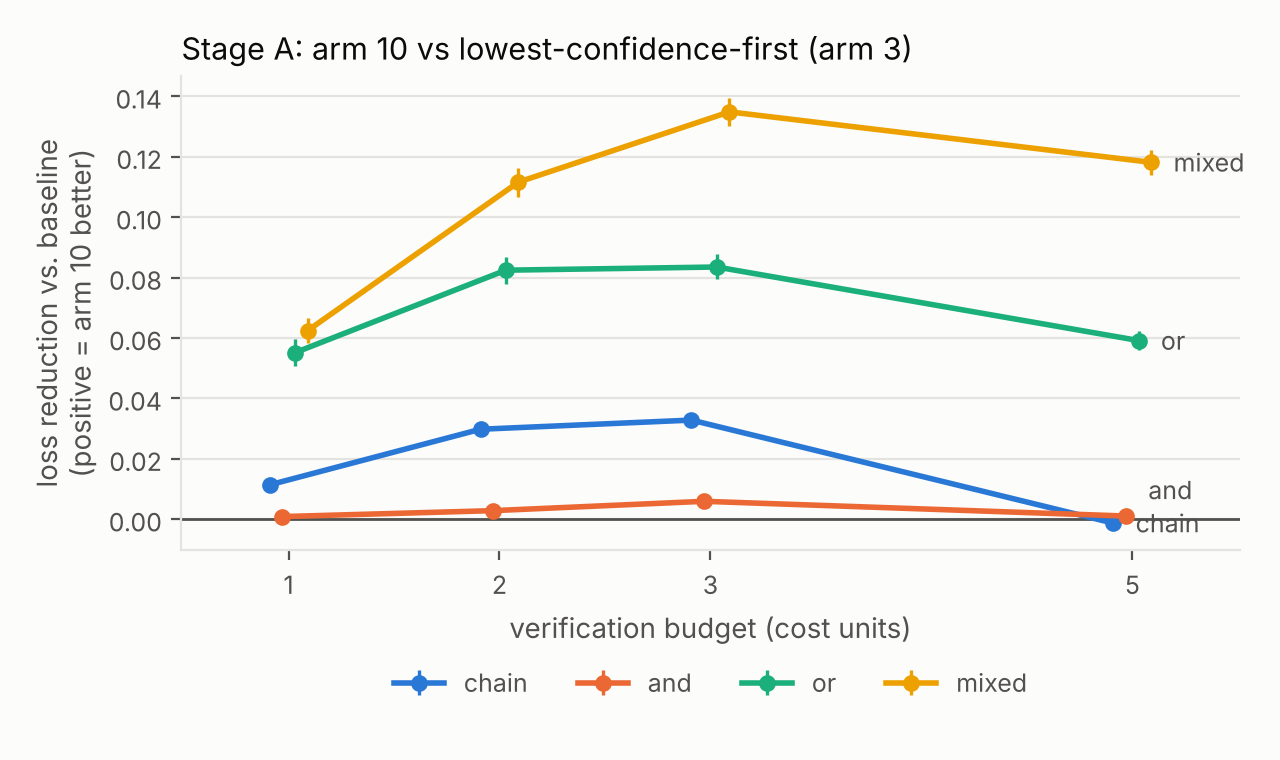
\includegraphics[width=.8\linewidth]{../results/figures/stageA_gain_vs_arm3.png}
\caption{Gain of arm 10 over lowest-confidence-first by structure and budget (95\% CIs).}
\end{figure}
\subsection{Stage B: noise robustness}
\begin{tabular}{lc}\toprule
Condition & Gain over arm 3 (95\% CI) \\\midrule
Clean & +0.077 [+0.070, +0.085] \\
ECE 0.10, verifier 5\% & +0.065 [+0.052, +0.077] \\
\bottomrule\end{tabular}

\subsection{Stage C: LLM behaviour on ProofWriter and PrOntoQA}
% Not yet run (API budget pending approval).

\section{Limitations}
% Exact enumeration ($n\le 20$); synthetic priors; generator-specific effects;
% Stage C pending; verifier error model independent given $Z$.

\section{Conclusion}

\end{document}
